La función para otorgar un valor a las celdas del terreno de batalla
para el caso del centro de extracción, es la misma que para cuando ya
se ha colocado el centro de extracción. Es decir, puntuar con mayor
puntuación el centro del tablero y disminuir según se aleje en
cualquiera de los cuatro sentidos.

A continuación la función en concreto:

\lstset{language=C++, texcl=true}
\begin{lstlisting}[frame=single]
float cellValue(int row, int col, bool** freeCells, int nCellsWidth, int nCellsHeight,
                float mapWidth, float mapHeight, List<Object*> obstacles, List<Defense*> defenses,
                bool isBase = false)
{
    try // Por si acaso freeCells no es del tamaño esperado, se recoje la excepcion y se devuelve una valoracion negativa
    {
        if (row >= 0 && col >= 0) // Comprueba si la fila y columna es mayor que cero
        {
            if(row < nCellsWidth && col < nCellsHeight) // Comprueba que la fila y columna este dentro de los margenes del trablero
            {
                if(freeCells[row][col]) // Comprobacion si el centro de la celda esta disponible
                {
                    int celdaCentroY = nCellsWidth / 2;
                    int celdaCentroX = nCellsHeight / 2;

                    float a = 0.0; // Valoracion de la casilla central en el eje Y
                    if(row >= celdaCentroY)
                        a = celdaCentroY*2 - row;
                    else if(row < celdaCentroY)
                        a = row;

                    float b = 0.0; // Valoracion de la casilla central en el eje X
                    if(col >= celdaCentroX)
                        b = celdaCentroX*2 - col;
                    else if(col < celdaCentroX)
                        b = col;

                    return a * b; // La mejor valoracion es el centro del tablero
                } else return 0.0;
            }
        }
    } catch(std::exception &e) {}
    return -1; // Por si se manda a valorar una celda que no esta dentro del tablero
}
\end{lstlisting}

% Elimine los símbolos de tanto por ciento para descomentar las siguientes instrucciones e incluir una imagen en su respuesta. La mejor ubicación de la imagen será determinada por el compilador de Latex. No tiene por qué situarse a continuación en el fichero en formato pdf resultante.
\begin{figure}
\centering
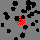
\includegraphics[width=0.7\linewidth]{./game} % no es necesario especificar la extensión del archivo que contiene la imagen
\caption{Estrategia devoradora para la mina}
\label{fig:defenseValueCellsHead}
\end{figure}
